\let\lesson\undefined
\newcommand{\lesson}{\phantomlesson{Bài 21.}}
\setcounter{section}{2}

\section{Trắc nghiệm nhiều phương án lựa chọn}
\setcounter{ex}{0}
\Opensolutionfile{ans}[ans/VN10-Y24-PH-SYL-032P-TN]
% ===================================================================
\begin{ex}\mkstar{1}
Điều nào sau đây là \textbf{đúng} khi nói về lực tác dụng lên vật chuyển động tròn đều?	
	\choice
	{Ngoài các lực cơ học, vật còn chịu thêm tác dụng của lực hướng tâm}
	{\True Hợp lực của tất cả các lực tác dụng lên vật đóng vai trò là lực hướng tâm}
	{Vật chỉ chịu tác dụng của lực hướng tâm}
	{Hợp lực của tất cả các lực tác dụng lên vật nằm theo phương tiếp tuyến với quỹ đạo tại điểm khảo sát}
	\loigiai{}
\end{ex}
% ===================================================================
\begin{ex}\mkstar{1}
	Trong chuyển động tròn đều, lực hướng tâm
	\choice
	{\True vuông góc với vector vận tốc}
	{cùng phương, cùng chiều với vector vận tốc}
	{cùng phương, ngược chiều với vector vận tốc}
	{có hướng không đổi}
	\loigiai{}
\end{ex}
% ===================================================================
\begin{ex}\mkstar{2}
Một xe đua chạy quanh một đường tròn nằm ngang, bán kính $R$. Tốc độ của xe không đổi. Lực đóng vai trò là lực hướng tâm lúc này là	
	\choice
	{lực đẩy của động cơ}
	{lực hãm}
	{\True lực ma sát nghỉ}
	{lực của vô – lăng (tay lái)}
	\loigiai{}
\end{ex}
% ===================================================================
\begin{ex}\mkstar{2}
Một vật đang chuyển động tròn đều dưới tác dụng của lực hướng tâm $F$. Nếu bán kính quỹ đạo tăng gấp hai lần so với trước và đồng thời giảm tốc độ quay còn một nửa thì so với ban đầu, lực hướng tâm	
	\choice
	{\True giảm 8 lần}
	{giảm 4 lần}
	{giảm 2 lần}
	{không thay đổi}
	\loigiai{Ta lập tỉ lệ:
		$$\dfrac{F_\text{ht 1}}{F_\text{ht 2}} = \dfrac{v_1 ^2 r_2}{v_2 ^2 r_1} = 8$$
		Vậy lực hướng tâm giảm 8 lần.}
\end{ex}
% ===================================================================
\begin{ex}\mkstar{2}
	Khi ô tô chuyển động đều trên một đoạn đường có dạng cung tròn, lực tác dụng đóng vai trò lực hướng tâm là
	\choice
	{trọng lực của ô tô}
	{phản lực của mặt đường}
	{\True hợp lực của tất cả các lực tác dụng lên xe}
	{lực ma sát giữa bánh xe và mặt đường}
	\loigiai{Khi ô tô chuyển động đều trên một đoạn đường có dạng cung tròn, lực tác dụng đóng vai trò lực hướng tâm là hợp lực của tất cả các lực tác dụng lên xe.}
\end{ex}
% ===================================================================
\begin{ex}\mkstar{2}
	Một xe đua chạy quanh một đường tròn nằm ngang, bán kính $\SI{250}{\meter}$. Tốc độ của xe không đổi có độ lớn là $\SI{50}{\meter/\second}$. Khối lượng xe là 2 tấn. Độ lớn của lực hướng tâm của chiếc xe là
	\choice
	{$\SI{10}{\newton}$}
	{$\SI{4E2}{\newton}$}
	{$\SI{4E3}{\newton}$}
	{\True $\SI{2E4}{\newton}$}
	\loigiai{Độ lớn của lực hướng tâm của chiếc xe:
		$$F_\text{ht}=ma_\text{ht}=m\dfrac{v^2}{R}$$
		$$\Rightarrow F_\text{ht}=\left(\SI{2E3}{\kilogram}\right)\cdot\dfrac{\left(\SI{50}{\meter/\second}\right)^2}{\SI{250}{\meter}}=\SI{2E4}{\newton}.$$}
\end{ex}
% ===================================================================
\begin{ex}\mkstar{2}
Một vật nhỏ khối lượng $\SI{250}{\gram}$ chuyển động tròn đều trên quỹ đạo tròn bán kính $\SI{1.2}{\meter}$. Biết trong 1 phút vật quay được 120 vòng. Độ lớn lực hướng tâm gây ra chuyển động tròn của vật là	
	\choice
	{\True $\SI{47.3}{\newton}$}
	{$\SI{3.8}{\newton}$}
	{$\SI{4.5}{\newton}$}
	{$\SI{46.4}{\newton}$}
	\loigiai{Tốc độ góc trong chuyển động của vật nhỏ:
		$$\omega=2\pi f=2\pi\cdot\left(\dfrac{120}{\SI{60}{\second}}\right)=\xsi{4\pi}{\radian/\second}$$
		Độ lớn lực hướng tâm gây ra chuyển động tròn của vật:
		$$F_\text{ht}=m\omega^2R=\left(\SI{0.25}{\kilogram}\right)\cdot\left(\xsi{4\pi}{\radian/\second}\right)^2\cdot\left(\SI{1.2}{\meter}\right)\approx\SI{47.3}{\newton}.$$}
\end{ex}
% ===================================================================
\begin{ex}\mkstar{2}
Hai quả cầu $m_1=2m_2$ nối với nhau bằng dây dài $\ell=\SI{12}{cm}$ có thể chuyển động không ma sát trên một trục nằm ngang qua tâm của hai quả cầu. Cho hệ quay đều quanh trục thẳng đứng. Biết hai quả cầu đứng yên không trượt trên trục ngang. Tìm khoảng cách từ hai quả cầu đến trục quay.	
	\choice
	{$r_1=\SI{5}{\centi\meter}$, $r_2=\SI{8}{\centi\meter}$}
	{\True $r_1=\SI{4}{\centi\meter}$, $r_2=\SI{8}{\centi\meter}$}
	{$r_1=\SI{4}{\centi\meter}$, $r_2=\SI{6}{\centi\meter}$}
	{$r_1=\SI{4}{\centi\meter}$, $r_2=\SI{10}{\centi\meter}$}
	\loigiai{Các quả cầu chuyển động quanh trục có khoảng cách đến tâm khác nhau, nhưng tốc độ góc thì vẫn như nhau. Lực căng dây đóng vai trò lực hướng tâm.\\
		Ta có:
		$$m_1 \omega^2 r_1 = m_2 \omega^2 r_2 \Rightarrow m_1 r_1 = m_2 r_2$$
		Mà $$r_1+r_2 = \ell$$
		Suy ra: $r_1 = \SI{4}{cm}$, $r_2 = \SI{8}{cm}$.}
\end{ex}
% ===================================================================
\begin{ex}\mkstar{3}
Biết khối lượng của Trái Đất là $M = \SI{6E24}{\kilogram}$. Chu kì quay của Trái Đất quanh trục của nó là $\SI{24}{\hour}$. Hằng số hấp dẫn $G=\SI{6.67E-11}{\newton\meter^2/\kilogram^2}$. Khoảng cách giữa tâm vệ tinh địa tĩnh của Trái Đất với tâm Trái Đất bằng	
	\choice
	{$\SI{422980}{\kilo\meter}$}
	{\True $\SI{42298}{\kilo\meter}$}
	{$\SI{42982}{\kilo\meter}$}
	{$\SI{42982}{\meter}$}
	\loigiai{Lực hấp dẫn do Trái Đất tác dụng lên vệ tinh địa tĩnh đóng vai trò là lực hướng tâm:
		$$G\dfrac{Mm}{R^2}=m\omega^2R\Leftrightarrow G\dfrac{M}{R^2}=\left(\dfrac{2\pi}{T}\right)^2R$$
		$$\Rightarrow R=\sqrt[3]{\dfrac{GM}{\left(\dfrac{2\pi}{T}\right)^2}}=\sqrt[3]{\dfrac{\left(\SI{6.67E-11}{\newton\meter^2/\kilogram^2}\right)\cdot\left(\SI{6E24}{\kilogram}\right)}{\left(\dfrac{2\pi}{24\cdot\SI{3600}{\second}}\right)^2}}\approx\SI{42297.5E3}{\meter}=\SI{42297.5}{\kilo\meter}.$$}
\end{ex}
% ===================================================================
\begin{ex}\mkstar{3}
	Một vật nặng có khối lượng $\SI{4}{\kilogram}$ được buộc vào đầu một sợi dây dài $L=\SI{1.2}{\meter}$. Người ta dùng một máy cơ để quay đầu còn lại của dây sao cho vật nặng chuyển động tròn đều trên mặt phẳng nằm ngang. Biết lực căng tối đa để dây không đứt có giá trị bằng $\SI{300}{\newton}$. Để dây không đứt, vật được phép quay với tốc độ tối đa là
	\choice
	{$\SI{7.91}{\text{vòng}/\second}$}
	{\True $\SI{1.26}{\text{vòng}/\second}$}
	{$\SI{2.52}{\text{vòng}/\second}$}
	{$\SI{1.58}{\text{vòng}/\second}$}
	\loigiai{Lực căng dây đóng vai trò là lực hướng tâm:
		$$\vec T=m\vec a_\text{ht}$$
		Chiếu phương trình trên lên phương bán kính, chiều dương hướng vào tâm quỹ đạo:
		$$T=m\omega^2 L$$
		Để dây không đứt thì
		$$T\le T_\text{giới hạn}$$
		$$\Leftrightarrow m\omega^2L\le T_\text{giới hạn}$$
		$$\omega\le\sqrt{\dfrac{T_\text{giới hạn}}{mL}}=\sqrt{\dfrac{\SI{300}{\newton}}{\left(\SI{1.2}{\meter}\right)\cdot\left(\SI{4}{\kilogram}\right)}}=\SI{7.91}{\radian/\second}.$$}
\end{ex}
\Closesolutionfile{ans}
\section{Trắc nghiệm đúng/sai}
\setcounter{ex}{0}
\Opensolutionfile{ans}[ans/VN10-Y24-PH-SYL-032P-TF]
% ===================================================================
\begin{ex}\mkstar{2}
\immini{	Vinasat-1 là vệ tinh viễn thông \textit{địa tĩnh} đầu tiên của Việt Nam được phóng vào vũ trụ năm 2008. Biết khối lượng của vệ tinh là $m=\SI{2.7}{\text{tấn}}$ và vệ tinh có quỹ đạo chuyển động nằm trong mặt phẳng xích đạo cách tâm Trái Đất $\SI{42000}{\kilo\meter}$. Biết vệ tinh được gọi là \textit{địa tĩnh} khi nó có chu kì quay quanh tâm Trái Đất bằng với chu kì tự quay của Trái Đất là $\SI{24}{\hour}$.}
{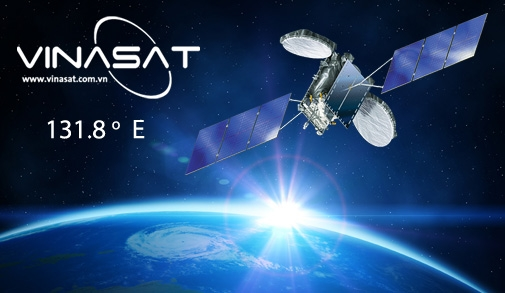
\includegraphics[scale=0.3]{../figs/VN10-2023-PH-TP032-P-4}}
	\choiceTF[t]
	{\True Tốc độ góc của vệ tinh bằng $\SI{7.27E-5}{\radian/\second}$}
	{\True Tốc độ dài của vệ tinh bằng $\SI{3054}{\meter/\second}$}
	{\True Gia tốc hướng tâm của vệ tinh bằng $\SI{0.22}{\meter/\second^2}$}
	{\True Lực hướng tâm tác dụng lên vệ tinh bằng $\SI{594}{\newton}$}
	\loigiai{
	\begin{itemchoice}
		\itemch Đúng. $\omega=\dfrac{2\pi}{T}=\SI{7.27E-5}{\radian/\second}$.
		\itemch Đúng. $v=\omega r=\SI{3054}{\meter/\second}$.
		\itemch Đúng. $a=\omega^2r=\SI{0.22}{\meter/\second^2}$.
		\itemch Đúng. $F_{\text{ht}}=ma_{\text{ht}}=\SI{594}{\newton}$.
	\end{itemchoice}
	}
\end{ex}
% ===================================================================
\begin{ex}\mkstar{2}
\immini{Đặt một vật có khối lượng $m=\SI{500}{\gram}$ lên một chiếc bàn cách tâm quay O của bàn $\SI{5}{\centi\meter}$. Cho bàn quay đều xung quanh tâm O với tốc độ góc $\xsi{\pi}{\radian/\second}$. Lấy $g=\SI{10}{\meter/\second^2}$.}
{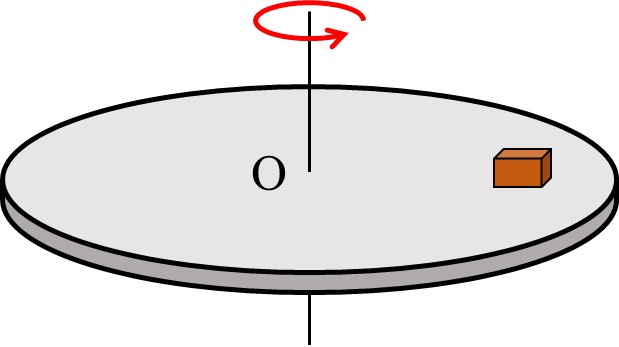
\includegraphics[scale=0.3]{../figs/VN10-2023-PH-TP032-P-5}}
	\choiceTF[t]
	{Nếu vật chuyển động quay cùng với bàn (không trượt trên bàn) thì trọng lực đóng vai trò lực hướng tâm}
	{Nếu vật chuyển động quay cùng cùng với bàn (không trượt trên bàn) thì chu kì quay của nó là $\SI{1}{\second}$}
	{Nếu vật quay cùng với bàn (không trượt trên bàn) thì lực hướng tâm tác dụng lên vật là $\SI{2}{\newton}$}
	{Nếu bàn quay với tốc độ $\SI{1}{\text{vòng/\second}}$ thì vật bị văng ra khỏi bàn. Biết hệ số ma sát nghỉ cực đại giữa vật và bàn là 0,2}
	\loigiai{
	\begin{itemchoice}
		\itemch Sai. Lực ma sát nghỉ giữa vật và bàn đóng vai trò lực hướng tâm.
		\itemch Sai. Chu kì quay là $T=\dfrac{2\pi}{\omega}=\SI{2}{\second}$.
		\itemch Sai. $F_{\text{ht}}=m\omega^2R=\SI{0.25}{\newton}$.	
		\itemch Sai. Để vật không trượt trên bàn thì $F_{\text{ht}}\le F_{\text{msn} \max}\Leftrightarrow m\omega^2R\le \mu mg\Leftrightarrow \omega\le\sqrt{\dfrac{\mu g}{R}}=\xsi{2\sqrt{10}}{\radian/\second}\approx\SI{1.01}{\text{vòng}/\second}$.
	\end{itemchoice}
	}
\end{ex}
% ===================================================================
\begin{ex}\mkstar{3}
	Mặt Trăng là vệ tinh tự nhiên của Trái Đất. Coi Mặt Trăng chuyển động tròn đều trên đường tròn có tâm là tâm Trái Đất và bán kính $R=\SI{3.84E8}{\meter}$. Biết chu kì quay của Mặt Trăng quanh Trái Đất là $T=\SI{235E4}{\second}$.
	\choiceTF[t]
	{\True Lực hấp dẫn do Trái Đất tác dụng lên Mặt Trăng đóng vai trò là lực hướng tâm}
	{\True Tốc độ góc của Mặt Trăng trong chuyển động quay quanh Trái Đất gần bằng $\SI{2.67E-6}{\radian/\second}$}
	{\True Gia tốc hướng tâm của Mặt Trăng có độ lớn gần bằng $\SI{2.7E-3}{\meter/\second^2}$}
	{Trong thời gian 28 ngày, Mặt Trăng quay được 0,9 vòng quanh Trái Đất}
	\loigiai{}
\end{ex}
% ===================================================================
\begin{ex}\mkstar{3}
Một người đi xe đạp trên chiếc vòng xiếc tròn có bán kính $R=\SI{6.4}{\meter}$. Biết khối lượng tổng cộng của hệ người và xe là $\SI{80}{\kilogram}$. Lấy $g=\SI{10}{\meter/\second^2}$.
\begin{center}
	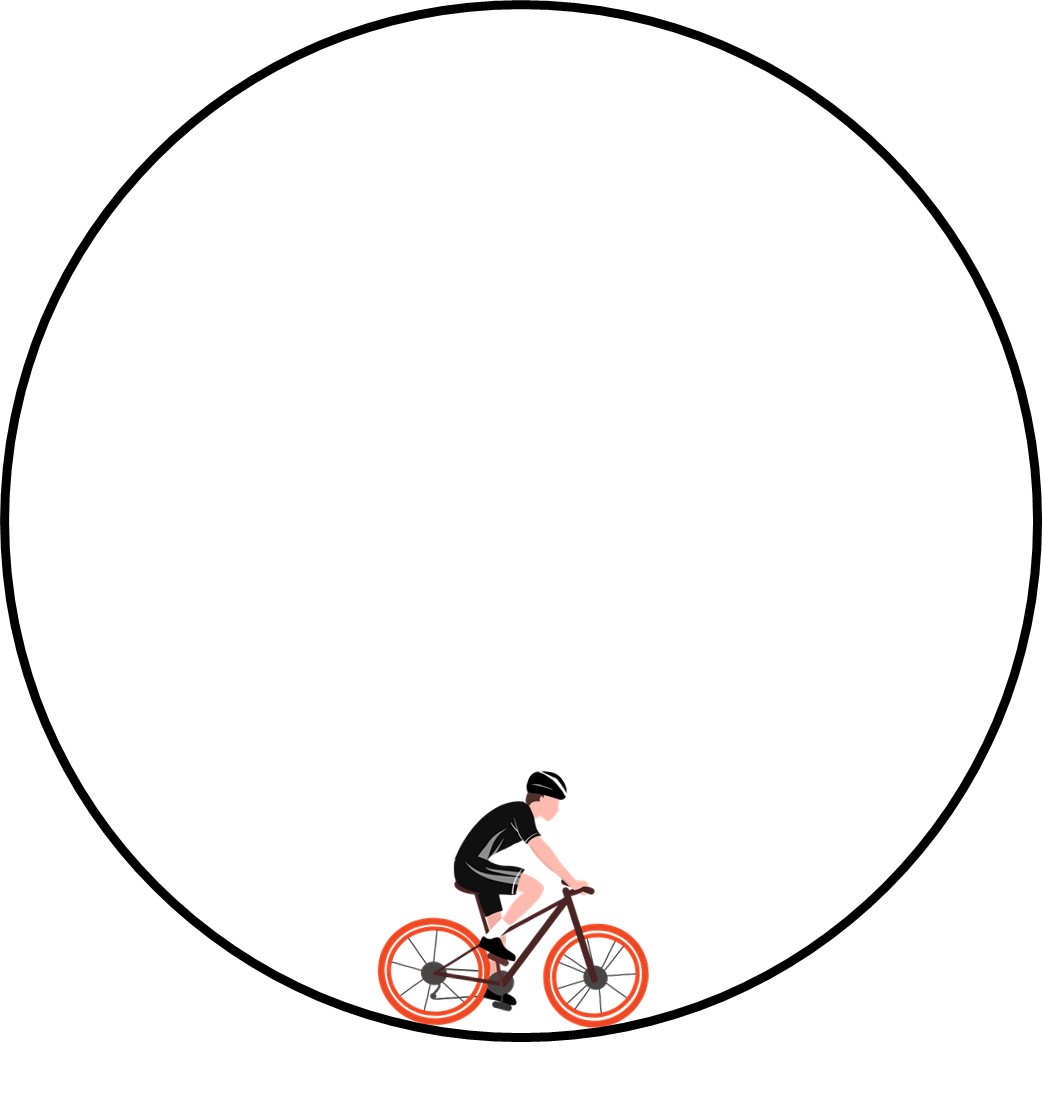
\includegraphics[scale=0.25]{../figs/VN10-2023-PH-TP032-P-6}
\end{center}
\choiceTF[t]
{Trọng lực tác dụng lên hệ đóng vai trò là lực hướng tâm}
{\True Áp lực của hệ lên vòng xiếc lớn nhất tại vị trí thấp nhất của vòng tròn}
{\True Vận tốc tối thiểu để xe đi qua điểm cao nhất của vòng xiếc mà không bị rơi bằng $\SI{8}{\meter/\second}$}
{Nếu xe qua điểm cao nhất với tốc độ $\SI{10}{\meter/\second}$ thì lực nén tác dụng lên vòng xiếc tại đó bằng $\SI{400}{\newton}$}
	\loigiai{}
\end{ex}
\Closesolutionfile{ans}
\section{Tự luận}
\setcounter{ex}{0}
\Opensolutionfile{ans}[ans/VN10-Y24-PH-SYL-032P-TL]
% ======================================================================
\begin{ex}\mkstar{2}
	Trạm không gian quốc tế ISS có tổng khối lượng 350 tấn, quay quanh Trái Đất ở độ cao $\SI{340}{km}$ nơi có gia tốc trọng trường $\SI{8,8}{m/s^2}$. Bán kính Trái Đất là $\SI{6400}{km}$. Tính độ lớn lực hướng tâm tác dụng lên trạm không gian.
	\loigiai{Lực hấp dẫn do Trái Đất tác dụng lên trạm không gian đóng vai trò là lực hướng tâm để trạm chuyển động tròn đều quanh Trái Đất.\\
		Lực hướng tâm tác dụng lên Trạm không gian:
		$$F = ma_\text{ht} = \left(\SI{350E3}{\kilogram}\right)\cdot\left(\SI{8.8}{\meter/\second^2}\right)=\SI{3080000}{\newton}.$$}
\end{ex}
% ======================================================================
\begin{ex}\mkstar{2}
	Một vật có $m = \SI{500}{g}$ chuyển động tròn đều trên đường tròn có $r = \SI{10}{cm}$. Lực hướng tâm tác dụng lên vật có độ lớn $\SI{5}{N}$. Tính tốc độ góc của vật.
	\loigiai{Ta có: 
		$$F_\text{ht} = mr\omega^2 \Rightarrow \omega = \SI{10}{rad/s}.$$}
\end{ex}
% ======================================================================
\begin{ex}\mkstar{3}
Một vật có khối lượng $m=\SI{20}{g}$ đặt ở mép một chiếc bàn quay. Hỏi phải quay bàn với tần số lớn nhất là bao nhiêu để vật không bị văng ra khỏi bàn? Cho biết mặt bàn hình tròn, bán kính $\SI{1}{m}$. Lực ma sát nghỉ cực đại bằng $\SI{0.08}{N}$.	
	\loigiai{Điều kiện để vật không bị văng ra khỏi bàn xoay là
		$$F_\text{ht} \leq F_\text{msn max}$$
		Trong đó: $F_\text{ht} = m\omega^2 r = m (2\pi f)^2 r$\\
		Và $F_\text{msn max} = \SI{0.08}{N}$\\
		Suy ra $$f^2 \leq \dfrac{F_\text{msn max}}{m 4 \pi ^2 r}\Rightarrow f\leq \SI{0.32}{\hertz}$$}
\end{ex}
% ======================================================================
\begin{ex}\mkstar{3}
	Một ô tô có khối lượng $\SI{1200}{\kilogram}$ chuyển động đều qua một đoạn cầu vượt (coi là cung tròn) với tốc độ $\SI{36}{\kilo \meter / \hour}$. Hỏi áp lực của ô tô vào mặt đường tại điểm cao nhất có độ lớn bằng bao nhiêu? Biết bán kính cong của đoạn cầu vượt là $\SI{50}{\meter}$. Lấy $g=\SI{10}{\meter / \second ^2}$.
	\loigiai{Các lực tác dụng lên vật: trọng lực $\vec P$, phản lực $\vec N$.\\
			Áp dụng định luật II Newton:
		$$\vec P + \vec N = m \vec a_\text{ht}.$$
		Chiếu phương trình định luật II Newton lên phương bán kính, chiều dương hướng vào tâm quỹ đạo:
		$$P-N=ma_\text {ht} \Rightarrow N=P-ma_\text{ht} = mg - m \dfrac{v^2}{r}.$$
		Thay số:
		$$N=\SI{1200}{\kilogram} \cdot \SI{10}{\meter / \second ^2} - \SI{1200}{\kilogram} \dfrac{(\SI{10}{\meter / \second})^2}{\SI{50}{\meter}} = \SI{9600}{\newton}.$$
		Vậy áp lực của ô tô vào mặt đường tại điểm cao nhất bằng $\SI{9600}{\newton}$.}
\end{ex}
% ======================================================================
\begin{ex}\mkstar{3}
Tiếp nối với câu 3. Nếu cầu võng xuống (các số liệu vẫn giữ như trên) thì áp lực của ô tô vào mặt cầu tại điểm thấp nhất có độ lớn là bao nhiêu?	
	\loigiai{Các lực tác dụng lên vật: trọng lực $\vec P$, phản lực $\vec N$.\\
		Áp dụng định luật II Newton:
		$$\vec P + \vec N = m \vec a_\text{ht}.$$
		Chiếu phương trình định luật II Newton lên phương bán kính, chiều dương hướng vào tâm quỹ đạo:
		$$N-P=ma_\text {ht} \Rightarrow N=P+ma_\text{ht} = mg + m \dfrac{v^2}{r}.$$
		Thay số:
		$$N=\SI{1200}{\kilogram} \cdot \SI{10}{\meter / \second ^2} + \SI{1200}{\kilogram} \dfrac{(\SI{10}{\meter / \second})^2}{\SI{50}{\meter}} = \SI{14400}{\newton}.$$
		Vậy áp lực của ô tô vào mặt cầu tại điểm thấp nhất bằng $\SI{14400}{\newton}$.}
\end{ex}
% ======================================================================
\begin{ex}\mkstar{3}
Một máy bay thực hiện một vòng bay trong mặt phẳng thẳng đứng. Bán kính vòng bay là $R= \SI{500}{m}$, tốc độ của máy bay có độ lớn không đổi $v=\SI{360}{km/h}$. Khối lượng của người phi công là $m=\SI{75}{kg}$. Lấy $g=\SI{10}{m/s^2}$. Xác định lực nén của người phi công lên ghế ngồi tại điểm cao nhất và thấp nhất của vòng bay.	
	\loigiai{Áp lực tại vị trí cao nhất:	
		$$N_\text{A} = F_\text{ht} - P = m \dfrac{v^2}{R} - mg =\SI{750}{N}.$$
		Áp lực tại vị trí thấp nhất:
		$$N_\text{B} = F_\text{ht} + P = m \dfrac{v^2}{R} + mg =\SI{2250}{N}.$$}
\end{ex}
% ======================================================================
\begin{ex}\mkstar{3}
Một chiếc xe đua có khối lượng $\SI{800}{\kilogram}$ chạy với tốc độ lớn nhất (mà không bị trượt) theo đường tròn nằm ngang có bán kính $\SI{80}{\meter}$ (hình vẽ) được một vòng sau khoảng thời gian $\SI{28.4}{\second}$. Lấy $g=\SI{9.8}{\meter/\second^2}$. Tính:
\begin{center}
	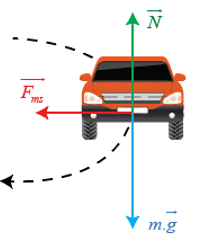
\includegraphics[width=0.25\linewidth]{../figs/VN10-2023-PH-TP032-P-1}
\end{center}
\begin{enumerate}[label=\alph*)]
	\item gia tốc hướng tâm của xe.
	\item hệ số ma sát nghỉ giữa các bánh xe và mặt đường.
\end{enumerate}	
	\loigiai{\begin{enumerate}[label=\alph*)]
			\item Xe đua chạy được một vòng trong khoảng thời gian $\SI{28.4}{\second}$ $\Rightarrow T=\SI{28.4}{\second}$.\\
			Tốc độ góc của xe:
			$$\omega=\dfrac{2\pi}{T}=\dfrac{2\pi}{\SI{28.4}{\second}}\approx\SI{0.22}{\radian/\second}$$
			Gia tốc hướng tâm của xe:
			$$a_\text{ht}=\omega^2 R=\left(\SI{0.22}{\radian/\second}\right)^2\cdot\left(\SI{80}{\meter}\right)\approx\SI{3.872}{\meter/\second^2}.$$
			\item Lực ma sát giữa xe và mặt đường đóng vai trò là lực hướng tâm giữa cho xe chuyển động trên đường tròn (không bị trượt):
			\begin{eqnarray*}
				&&F_\text{ht}=F_\text{msn}\le F_\text{msn max}\\
				&\Leftrightarrow& ma_\text{ht}\le \mu mg\\
				&\Rightarrow& \mu \ge \dfrac{a_\text{ht}}{g}=\dfrac{\SI{3.92}{\meter/\second^2}}{\SI{9.8}{\meter/\second^2}}=0,4
			\end{eqnarray*}
			Vậy để xe không bị trượt thì $\mu \ge 0,4$.
	\end{enumerate}}
\end{ex}
% ======================================================================
\begin{ex}\mkstar{3}
	Ở độ cao bằng một nửa bán kính của Trái Đất có một vệ tinh nhân tạo chuyển động tròn đều xung quanh Trái Đất. Biết gia tốc rơi tự do ở mặt đất là $g=\SI{10}{\meter/\second^2}$ và gia tốc rơi tự do ở độ cao $h$ so với mặt đất là $g_h=\dfrac{R^2\cdot g}{\left(R+h\right)^2}$; bán kính của Trái Đất là $\SI{6400}{\kilo\meter}$. Tính tốc độ của vệ tinh.
	\loigiai{Khoảng cách giữa vệ tinh và tâm Trái Đất:
		$$r=R+h=R+\dfrac{R}{2}=1,5R$$
		Gia tốc rơi tự do ở độ cao $h=\dfrac{R}{2}$:
		$$g_h=\dfrac{R^2}{\left(1,5R\right)^2}\cdot g=\dfrac{g}{1,5^2}$$
		Lực hấp dẫn do Trái Đất tác dụng lên vệ tinh đóng vai trò là lực hướng tâm giữ cho vệ tinh chuyển động tròn đều xung quanh Trái Đất:
		\begin{eqnarray*}
			&&F_\text{hd}=F_\text{ht}\\
			&\Leftrightarrow& mg_h=m\cdot\dfrac{v^2}{r}\\
			&\Leftrightarrow& g_h=\dfrac{v^2}{r}\\
			&\Rightarrow& v=\sqrt{\dfrac{gR}{1,5}}=\sqrt{\dfrac{\left(\SI{10}{\meter/\second^2}\right)\cdot\left(\SI{6400E3}{\meter}\right)}{1,5}}=\SI{6352}{\meter/\second}.
	\end{eqnarray*}}
\end{ex}
% ======================================================================
\begin{ex}\mkstar{4}
	Một vật nhỏ được buộc vào đầu một sợi dây có chiều dài $\SI{0.75}{\meter}$. Nếu quay đều và chậm, sợi dây quét thành một mặt nón (hình vẽ). Tính tần số quay để dây lệch góc $\alpha=\SI{60}{\degree}$ so với phương thẳng đứng, lấy $g=\SI{10}{\meter/\second^2}$.
	\begin{center}
		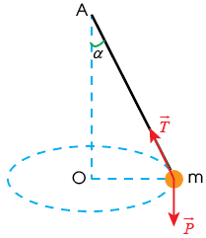
\includegraphics[width=0.25\linewidth]{../figs/VN10-2023-PH-TP032-P-2}
	\end{center}
	\loigiai{Hợp lực của trọng lực $\vec P$ và lực căng dây $\vec T$ đóng vai trò là lực hướng tâm
		$$\vec F_\text{ht}=\vec P+\vec T$$
		\begin{center}
			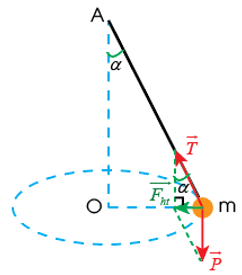
\includegraphics[width=0.25\linewidth]{../figs/VN10-2023-PH-TP032-P-3}
		\end{center}
		Ta có:
		\begin{eqnarray*}
			&&\tan \alpha=\dfrac{F_\text{ht}}{P}=\dfrac{m\omega^2r}{mg}=\dfrac{\omega^2\ell\sin\alpha}{g}\\
			&\Leftrightarrow& \tan \SI{60}{\degree}=\dfrac{\omega^2\cdot\left(\SI{0.75}{\meter}\right)\cdot\sin\SI{60}{\degree}}{\SI{10}{\meter/\second^2}}\\
			&\Rightarrow& \omega=\SI{5.16}{\radian/\second}\\
			&\Rightarrow& f=\dfrac{\omega}{2\pi}=\SI{0.82}{\hertz}.
	\end{eqnarray*}}
\end{ex}
\Closesolutionfile{ans}
